%\chapter[VLQ models]{Vector Like Quarks: Generic model}
%\label{chap:VLQ}
%
%From chapter~\ref{chap:SM} we have seen how there are some parts in the SM that does not work very well. From such internal issues some further models/theories have been developed. All this theories are commonly grouped under the term Beyond Standard Model or simply BSM. One of the most famous BSM theory is supersymmetry (SUSY). This theory postulates a symmetry that does not distinguish between fermions and bosons. This idea have given birth to a plethora of model realizations and physics predictions. So far, nothing of the new consequences of this theory have been confirmed but the experiments have an enormous investment on their search. But not only SUSY have seen the day light, there is on the market an astonishing amount of BSM theories addressing different issues of the SM. Extra dimensions, fourth families, composite Higgs are a few of them.
%
%In this chapter we will describe a bunch of models that introduce additional heavy quarks, heavier than the top, in order to solve the hierarchy problem, described on section~\ref{sec:hier}. 
%
%\section{Motivation}
%\label{sec:motiv}
%
%Why to introduce extra quarks.
%
%Plausible solution of hierarchy problem.
%
%Reference to models with extra quarks. (?)
%
%\section{Generic Formulation}
%\label{sec:form}
%
%Formalism: Generic Langranian. Description of mixings with SM quarks.
%
%\begin{table}[htbH]
%\label{tab:VLQRepre}
%\begin{center}
%\begin{tabular}{|c|c|c|}
%\hline 
%xxxxxxx & xxxxxxx & xxxxxxx
%\hline
%\end{tabular}
%\caption{Possible VLQ representations and correponding $SU(2)_{L}\times U(1)$ charges.}
%\end{center}
%\end{table}
%\begin{TOINCLUDE}Table with different possible representations and assigned charges\end{TOINCLUDE}
%
%\subsection{Production modes}
%\label{sec:prod}
%
%Description of pair and single production. Parallel to production modes of top. Comparison between cross sections for pair and single production.
%
%\begin{figure}[!Hhtbp]
%  \begin{center}
%    
\includegraphics[width=0.3\textwidth]{figs/CMSlogo.png}
%    \caption{Feynman diagrams of $T$ production in pairs [left] and single [right]}
%    \label{fig:ProdDiag}
%  \end{center}
%\end{figure}
%
%\begin{figure}[!Hhtbp]
%  \begin{center}
%    
\includegraphics[width=0.3\textwidth]{figs/CMSlogo.png}
%    \caption{$T$ production cross section for pair and single case as a function of $T$ mass for different center of mass energy in proton-proton collisions.}
%    \label{fig:TProdXS}
%  \end{center}
%\end{figure}
%\Begin{TOINCLUDE}Plot of production cross section at LHC for different energies as a function of the mass. Feynman diagrams of the production processes.\end{TOINCLUDE}
%
%\subsection{Decay modes}
%\label{sec:decay}
%
%Description of possible decay channels of $T$. Relative importance of decay channels depending on the mass. 
%
%\begin{figure}[!Hhtbp]
%  \begin{center}
%    
\includegraphics[width=0.3\textwidth]{figs/CMSlogo.png}
%    \caption{$T$ branching ratios as a function of its mass.}
%    \label{fig:TBRs}
%  \end{center}
%\end{figure}
%\begin{TOINCLUDE}Plot of branching ratio as a function of the mass for different scenarios (representations)\end{TOINCLUDE}

\chapter{Feasibility study for a search of a \Tp~at LHC at 8 TeV}
\label{chap:pheno}

In this chapter a strategy is developed to look for a \Tp~in the full hadronic final state. This channel is very challenging. Mainly because the number of expected events for backgrounds in the full hadronic channel is several orders of magnitude higher than the number of expected events for signal in proton-proton collisions at 8 TeV center of mass energy. Additionally, it is a channel poorly explored by current analysis due to its intrinsic difficulties, what makes this an original proposal. In section~\ref{chap:VLQ} a generic model of VLQ has been introduced. In addition some of their properties predictions have been described. As discussed, a \Tp~can be produced in proton-proton collisions at LHC in several ways. For \Tp~masses higher than 500~\GeVcc~single production mode gives a higher cross section with regard to pairwise production. Consequently, if there is a \Tp~in nature, it has a higher observability in data considering single production process. 

For example, with 20 $\text{fb}^{-1}$ at 8~TeV, around 4000 events are expected for a single produced \Tp~with a mass of 700~\GeVcc, whereas only 500 are expected in the pair production process. But, all these events split in all the possible different final states. In the case of a 700~\GeVcc~mass \Tp , the dominant decay channel is to top-Higgs, that is around 50\% from figure~\ref{fig:TBRs}. Following the calculation, this means about 2000 events are expected where the \Tp~decays into top and Higgs. In this study the choice of the mass value for the \Tp~is based on the argument that it could be accessible to run 1 data collected by CMS at 8 TeV center of mass energy. The principal objective of the study is to motivate a full data search for VLQ. However, it is clear that for higher masses, specially higher than 1 TeV, special techniques, different from the ones used in this study, will be necessary. For such energies, it will be perhaps needed to use for example boosted techniques~\cite{CMS:2013vca, ATLAS-CONF-2013-084, Usai:2015vva}. These techniques are useful when several decay products of a massive particle are merged in a single jet, because of its high $p_{T}$. They allow to recover underlying substructure of jets.

Finally, from Higgs branching ratios (figure~\ref{fig:HiggsBrs}), the Higgs decays the most of the times, 57\%, to a pair of $b$-quarks. Additionally, the top quark decays in a $b$-quark and a \W~boson with a branching ratio about 100\%. And the \W~boson decays into a pair of quarks 66\% of times. Using these three branching ratios, the $Br(T'\to 3b, 2j)=37$\%. Thus the expected number of events of \Tp~into 5 quarks (or jets) is of around 700 events. For collected events by the CMS experiment in LHC run 1, the full hadronic final state constitutes the channel with the highest number of expected events. In the following sections a tentative strategy to extract these events from backgrounds is described. A majority of the results exposed in this chapter are part of the reference~\cite{Beauceron:2014ila}. A data analysis inspired in this phenomenological study will be presented in chapter~\ref{chap:search}. %The main challenge in the full hadronic final state is to distinguish signal from the enormous quantity of expected background events. 

%Discussion on selection of full hadronic channel.

\section{Samples used in the study}
\label{sec:PhenoSam}

This feasibility study relied on Monte-Carlo simulations for the signal and backgrounds. MadGraph 5~\cite{Alwall:2014hca, Alwall:2011uj}, version 1.5.11, has been used for the generation of parton level samples. Signal model has been implemented with the FeynRules toolkit~\cite{Alloul:2013bka}. For the simulation of hadronization processes of parton samples, Pythia 6~\cite{Sjostrand:2006za} has been used. These tools are well known to describe correctly high jet multiplicity final states, specifically an unstable particle (as the \W~boson, \Z~boson or $t$-quark) with up to four additional jets. For a detailed description of Monte-Carlo techniques and tools see chapter~\ref{chap:MC}. 

The cross sections and expected number of events for signal and each background used in the study, at 8~TeV for 20~fb$^{-1}$, are listed in table~\ref{tab:xsec}. All SM processes giving a final state with at least 5 jets in the final state have been considered. As it will be described in the next section, the strategy of the study is based in the fully hadronic final state where the signal produce 5 jets coming from \Tp~and one additional jet in the forward region.

At production level some loose cuts were required to facilitate the sample generation. QCD was produced requiring all jets with a $p_{T}>30$~GeV/c and within a pseudo-rapidity of $|\eta|<5$. All the other background samples were produced with jets having $p_{T}>10$~GeV/c and no cut on the pseudo-rapidity. For samples with at least one \Z~boson, di--boson processes \Z\Z, \W\Z and \Z+jets, the mass of the di--lepton pair was required to satisfy $M_{ll}>50$~\GeVcc~in order to avoid integration troubles (when the di--lepton invariant mass approaches zero the cross-section diverges). After hadronization, the jets were built up with Anti-Kt algorithm using $R=0.5$ with the standard implementation provided by the FastJet package~\cite{Cacciari:2011ma}.

The signal sample was produced with jets with $p_{T}>10$~GeV/c with the same packages. The vector-like mass was set around 700~\GeVcc, and the mixing to their maximal allowed values when both mixing to third and first generation are allowed (however the couplings to light generations were maximized to the experimental constraints, the coupling to the second generation is negligible). This choice corresponds to the following set of parameters used in the simulation for the signal: $\xi_Z^{T}=0.5145$, $V_{R}^{41}=0.078$, $V_{R}^{42}=0.0041$, $\kappa_{T}=0.087$ and $BR(T' \to H^{0} t)=0.472$. With this choice, the physical mass of the \Tp~is $M_{T'}=734$~\GeVcc. This also set the cross section to 200~fb. These parameters correspond to a benchmark point similar to the one defined in~\cite{Cacciapaglia:2011fx}, it was set to obtain a VLQ mixed with light and heavy SM quark generations and a \Tp~mass close to 700~\GeVcc.

The samples used in this study were analyzed using MadAnalysis package~\cite{Conte:2012fm, Conte:2014zja}.

\section{Strategy for the full hadronic final state}
\label{sec:Pstra}

The final state of interest for this study, the full hadronic final state, contains 3 $b$-quarks and 2 additional quarks as decay products of the \Tp. Two $b$'s coming from the Higgs boson, a third $b$ from the top-quark decay, and 2 light jets from the \W~boson decay. In addition, the \Tp~is produced in association with a light quark. Figure~\ref{fig:ForwJ} shows the $\eta$ distribution of the jet produced in association with the \Tp. Consequently, the signal events are expected to have at least 6 jets, 5 with an \etal{2.5}~and one with an \etal{5}. Unlike the leptonic channels all the decay products of the \Tp~are seen by a detector (mainly produced with an \etal{2.5}), as CMS, circumstance that allows to do a full mas reconstruction of it.

\begin{figure}[!Hhtbp]
  \begin{center}
    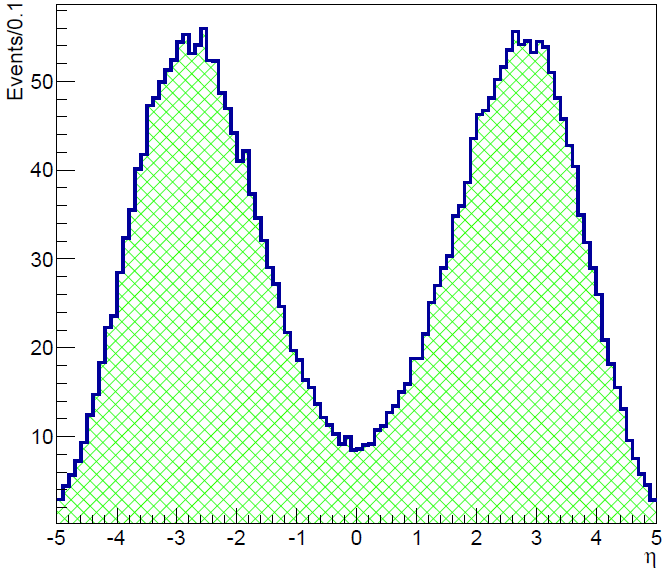
\includegraphics[width=0.45\textwidth]{figs/Pheno/SixthJet.png}
    \caption{$\eta$ distribution of the forward jet produced in association with the \Tp. Signal sample is normalized to theoretical cross section and to 20~$fb^{-1}$.}
    \label{fig:ForwJ}
  \end{center}
\end{figure}

The main difficulty in full hadronic final states is the large QCD background. In this study all the possible SM backgrounds giving a full hadronic final state were included, in decreasing order of contribution: QCD production, vector plus jets ($V$+jets, where $V$ is a \W~or a \Z~boson), \ttbar, single top, and di--boson (\W\W, \W\Z, \Z\Z) have been considered, as shown in table~\ref{tab:xsec}. 

\begin{table}[htbH]
\begin{center}
\begin{tabular}{||l|c|r||}
  \hline\hline
  Process & $\sigma_{\rm 8 TeV}$ (pb) & Expected Events \\ \hline
 Signal ($T'j$) & 0.2 & 700 \\
 \hline
  QCD (bbjjj) & 500 & 10,000,000 \\
  \W+jets & 37,509 & 750,180,000 \\
  \Z+jets & 3,503.71 & 70,074,200 \\ 
  \ttbar & 234 & 4,680,000 \\
  single-$t$ & 114.85 & 2,297,000 \\
  Di-boson & 96.82 & 1,936,400 \\
  \hline\hline
\end{tabular}
\caption{Cross sections and expected number of events for background processes and signal for a luminosity of 20~$fb^{-1}$. The single top and di-boson samples were produced with up to 3 additional jets. \label{tab:xsec}}
\end{center}
\end{table}

The analysis strategy relies on the correct identification of the 5 jets coming from the \Tp. For this purpose a jet association method has been designed to select the 5 jets from the \Tp~based on the characteristics of the signal. The method used to identify the jets coming from \Tp~is the following:
\begin{itemize}
\item Tag b--jets and keep events with at least two b-jets ($n_{b}\ge 2$).
\item To reconstruct the Higgs, only pairs of b-jets with a ${\Delta R_{bb} <2.5}$ are considered. If more than one pair is found, the pair with the closest mass to the Higgs boson mass (125~\GeVcc) is chosen. The two jets chosen for the Higgs reconstruction are not longer considered in the jet collection for the reconstruction procedure of the \W~boson and top quark.
\item From the remaining jets, the pair of jets with mass closest to the W-mass (80~\GeVcc) is identified as the \W~boson. 
\item Finally, from the remaining jets, a third jet is chosen and coupled to the previously identified W-jets. The jet giving the closest mass to the top mass (172~\GeVcc), combined with the W-jets, is selected as the top b-jet.
\end{itemize}

From the objects reconstructed with the jet association method and other signal characteristics, a selection to discriminate signal events from backgrounds has been designed. As in the SM backgrounds there is no real Higgs, the selection strongly relies on the presence of a real Higgs in signal events. Also the presence of a real top in signal events is used. 

In the following section, the selection applied is described. The different criteria have been chosen in order to increase the discrimination of signal from background. The objective of the study is not to obtain the best possible discrimination but moreover to illustrate a possible selection to extract the signal and to give a qualitative understanding of signal characteristics.
%General discussion of strategy used for selection. 

\section{Event selection}
\label{sec:Psel}

%Description of selection. Paragraph per variable.
All cuts were applied one after the other in the order given in the following list:

\begin{itemize}

\item \textit{Cut 0}: In first instance only the events with at least 6 jets with ${p_T > 30}$~GeV/c are kept. From them, at least five jets within $|\eta|<2.5$ and at least one jet within $2<|\eta|<5$. The \Tp~decays into five central jets, but the associated jet produced with it tends to be in the forward direction, as shown in figure~\ref{fig:ForwJ}. This cut tries to mimic the detector acceptance.

\item \textit{Cut 1}: The first kinematic cut requires ${p_{T}>150}$~GeV/c for the leading jet, ${p_{T}>80}$~GeV/c for the sub-leading jet and ${p_{T}>60}$~GeV/c for the 3$^{rd}$ and 4$^{th}$ leading jets in each event. The \pt~distribution of the six leading jets is shown in figure~\ref{fig:Var1}.

\begin{figure}[!Hhtbp]
  \begin{center}
    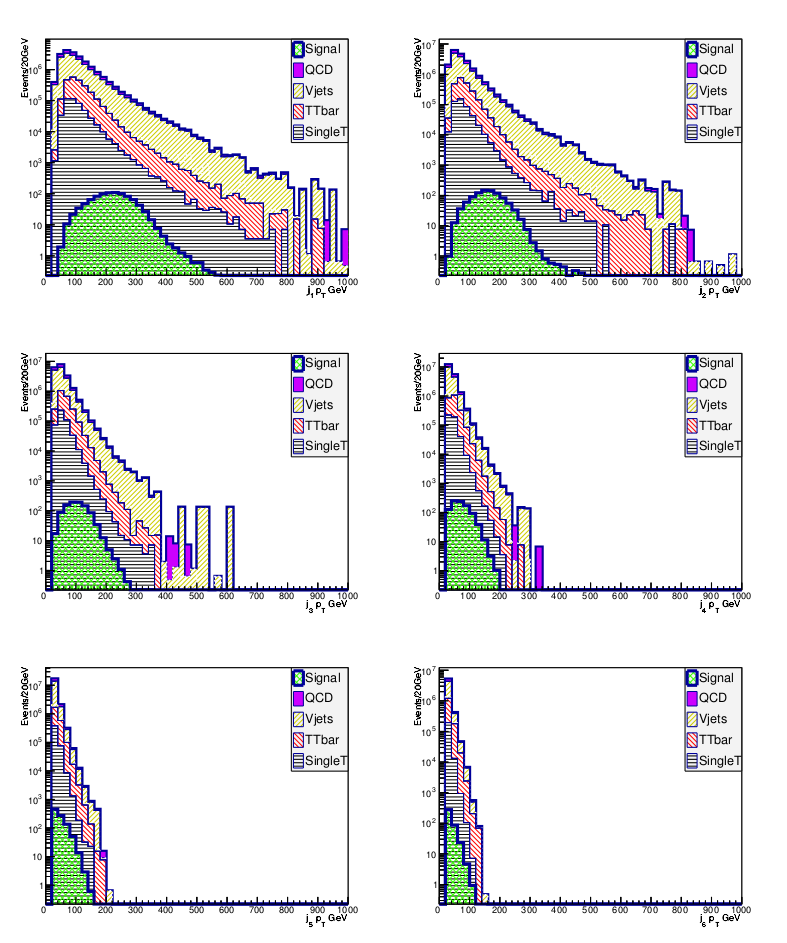
\includegraphics[width=0.95\textwidth]{figs/Pheno/JetPt.png}
    \caption{$p_{T}$  of the six leading jets for backgrounds (stacked) and signal (over--imposed) normalized to 20 $fb^{-1}$ luminosity. QCD background is on top of the stack of backgrounds.}
    \label{fig:Var1}
  \end{center}
\end{figure}

\item \textit{Cut 2}: The following criteria uses the total hadronic energy ($H_{T}=\sum |p_{T}(j)|$, with the sum over all jets in the event), which is plotted in figure~\ref{fig:Var2} for each backgrounds and the signal. Signal events have higher \HT~than background events, reflecting the presence of the very massive \Tp. Events with $H_{T}>630$~GeV/c were selected.

\begin{figure}[!Hhtbp]
  \begin{center}
    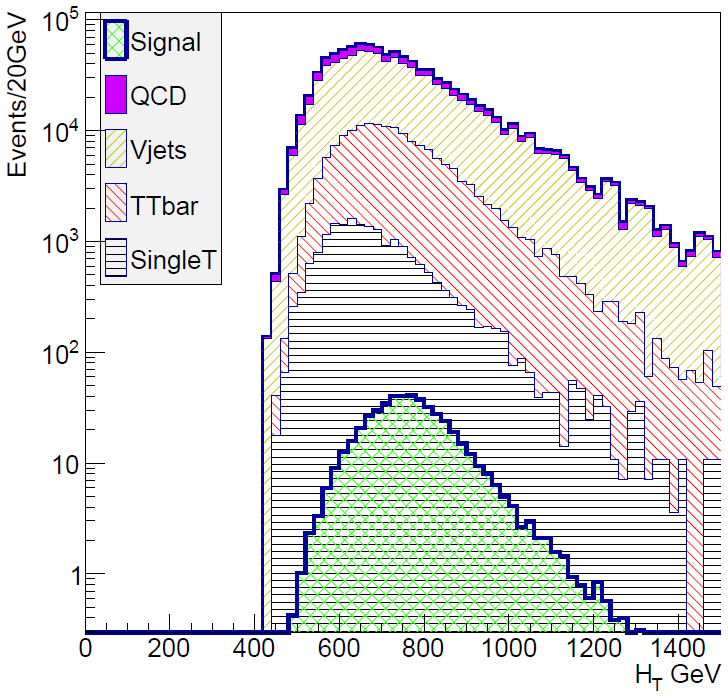
\includegraphics[width=0.45\textwidth]{figs/Pheno/HT.png}
    \caption{Total hadronic energy for backgrounds (stacked) and signal (over--imposed) normalized to 20~$fb^{-1}$ luminosity. $H_{T}$ is higher in signal than in background events.}
    \label{fig:Var2}
  \end{center}
\end{figure}

\item \textit{Cut 3}: At least two b-jets were required in order to perform the jet association procedure. The identification of jets coming from b-quarks has been described in section~\ref{sec:bid}. However, as this study has been done up to the hadronization level, the same techniques were not used. As a substitute, the following method was used to emulate the performance of b-jet identification algorithms:
  \begin{enumerate}
  \item Select a working point for a b-tagging algorithm. This sets the efficiency of the algorithm to tag jets coming from a b-quark ($\epsilon^{b-tag}_{b}$), from a c-quark ($\epsilon^{b-tag}_{c}$) and from a light-quark ($\epsilon^{b-tag}_{l}$). As reference, the loose working point of the CSV algorithm has been chosen (discussed in section~\ref{sec:bid}). The CMS results~\cite{CMS-PAS-BTV-13-001} were used: $\epsilon^{b-tag}_{b}=0.9$, $\epsilon^{b-tag}_{c}=0.6$ and $\epsilon^{b-tag}_{l}=0.1$. 
  \item Throw a random number $r$ between 0 and 1 for each event.
  \item Loop over all the jets from an event and, depending on their flavor and the random number from last step, declare each jet to be or not to be b-tagged. A jet is b-tagged if: it is coming from a b-quark and $r\leq\epsilon^{b-tag}_{b}$, or it is coming from a c-quark and $r\leq\epsilon^{b-tag}_{c}$, or it is coming from a light-quark and $r\leq\epsilon^{b-tag}_{l}$.
  \end{enumerate}

The number of b-tagged jets using the method described above is displayed in figure~\ref{fig:Nbs}.

\begin{figure}[!Hhtbp]
  \begin{center}
    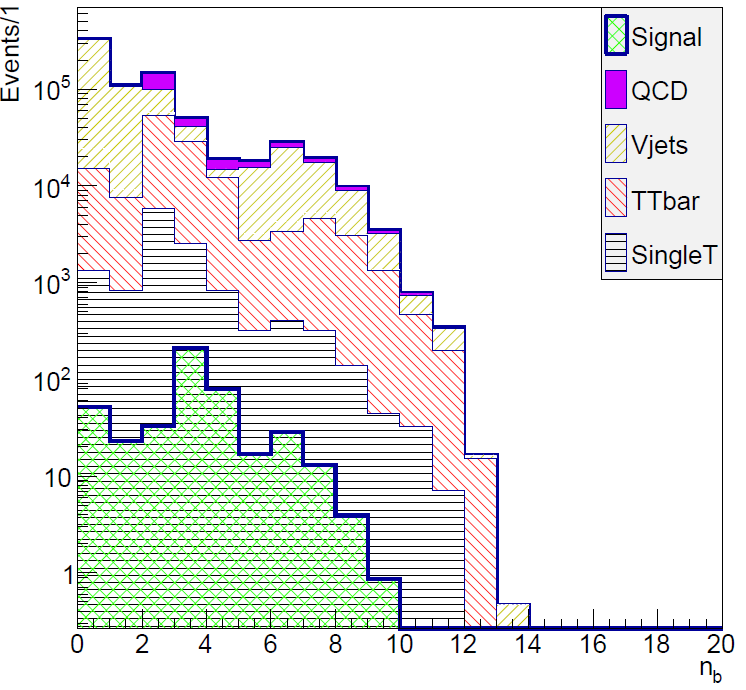
\includegraphics[width=0.45\textwidth]{figs/Pheno/Nb.png}
    \caption{B-tagged jet multiplicity for backgrounds (stacked) and signal (over--imposed) normalized to 20~$fb^{-1}$ luminosity. The signal has as mean value 3 b-tagged jets.}
    \label{fig:Nbs}
  \end{center}
\end{figure}

\item \textit{Cut 4}: Events are kept if the two jets assigned to the Higgs have a $\Delta R_{bb}<1.8$. As the Higgs boson comes from the decay of the massive \Tp, it is produced with a momentum different from zero. As a result the two b's from the Higgs boson are produced close by in $\eta-\phi$ space.

\item \textit{Cut 5}: As the Higgs boson and top quark produced by the signal come from a very heavy particle, they are expected to have a greater $p_{T}$ than fakes reconstructed in backgrounds. Accordingly, only events which have a Higgs candidate with $p_{T}>200$~GeV/c and a top candidate with $p_{T}>300$~GeV/c were selected. The $p_{T}$ of the reconstructed Higgs candidate and top quark candidate for signal and backgrounds are shown in figure~\ref{fig:HptToppt}, in a 2D histogram.

\begin{figure}[!Hhtbp]
\begin{center}
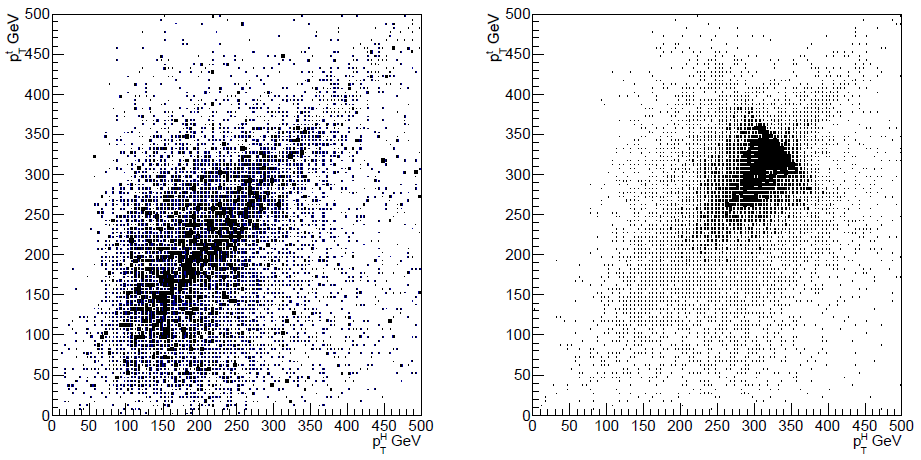
\includegraphics[width=0.9\textwidth]{figs/Pheno/HPTTPT.png}
\caption{Reconstructed Higgs candidate $p_{T}$ in the x axis and reconstructed top candidate $p_{T}$ in the y axis for backgrounds (left) and signal (right). Signal events have reconstructed Higgs and top with higher \pt~than backgrounds.
\label{fig:HptToppt}}
\end{center}
\end{figure}

\item \textit{Cut 6}: The distance in $\eta-\phi$ plane between the reconstructed \W~and Higgs candidates is preferentially around 3 for signal, while for backgrounds the distribution is much more spread as there is no real Higgs boson. $\Delta R_{HW}$ is plotted in figure~\ref{fig:Var3}. Selecting only the events within $2.2<\Delta R_{HW}<3.5$ helps to reduce QCD and~\W+jets~background~events.

\begin{figure}[!Hhtbp]
  \begin{center}
    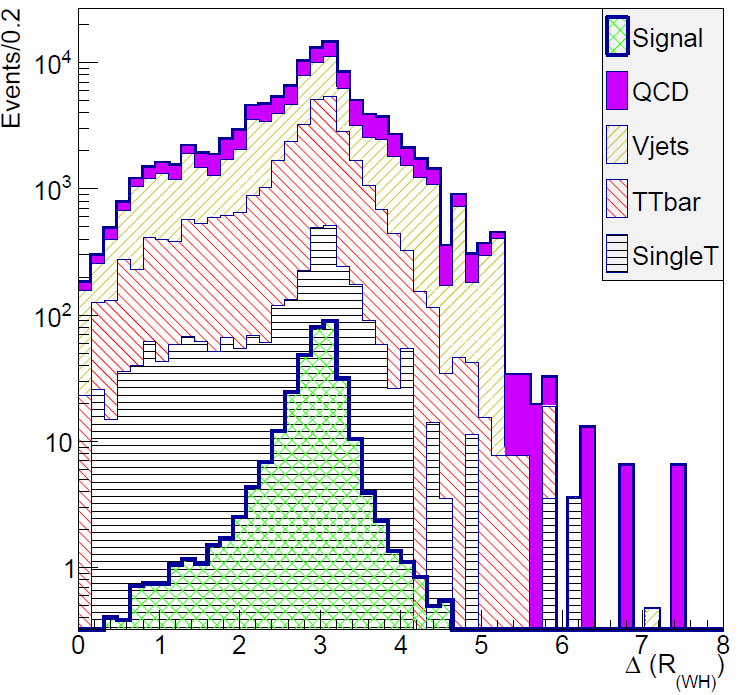
\includegraphics[width=0.45\textwidth]{figs/Pheno/DRWH.png}
    \caption{$\Delta R$ between the reconstructed Higgs and \W~candidates for backgrounds (stacked) and signal (over--imposed) normalized to 20 $fb^{-1}$ luminosity. Although signal and backgrounds have a mean value of $\Delta R_{HW}=3$, backgrounds tend to have lower values than signal, as well as larger tails.}
    \label{fig:Var3}
  \end{center}
\end{figure}

\item \textit{Cut 7}: The $\Delta \phi_{bb}$ of the b jets identified as coming from the Higgs boson candidate and the $\Delta \phi_{bW}$ between the reconstructed W candidate and the jet which formed the top are expected to be mainly close in $\phi$ for the signal while more evenly distributed for backgrounds. Only events with $\Delta \phi_{bb}<2.0$ and $\Delta \phi_{bW}<3.3$ were kept. This cut is specially useful for reducing QCD and \W+jets background events.

\item \textit{Cut 8}: As in cut 7, the \W~boson produced from the \Tp~is expected to have a non-zero momentum. Thus, the $\Delta \phi_{jj}$ between the jets of the \W~boson are expected to be more centered around zero for the signal with respect to the backgrounds. Events were required to have $\Delta \phi_{jj}<2.3$ to reduce single--top background.

\item \textit{Cut 9}: Events with a reconstructed Higgs mass close to the Higgs mass were kept. Events with a Higgs candidate with a mass between $100$~\GeVcc~and $135$~\GeVcc~were selected for the analysis. The distribution of the reconstructed Higgs mass is shown in figure~\ref{fig:Var4}.

\begin{figure}[!Hhtbp]
  \begin{center}
    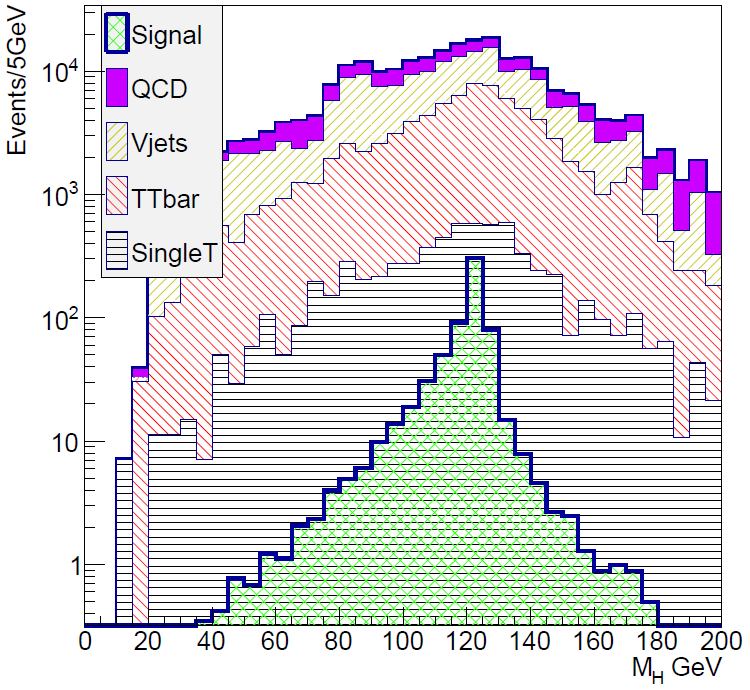
\includegraphics[width=0.45\textwidth]{figs/Pheno/MH.png}
    \caption{Mass of the reconstructed Higgs candidate for backgrounds (stacked) and signal (over--imposed). Backgrounds have larger tails than signal for the reconstructed Higgs mass.}
    \label{fig:Var4}
  \end{center}
\end{figure}

\item \textit{Cut 10}: For the final cut the relative total hadronic energy is defined as the ratio between the $p_{T}$ of the decay products identified as the Higgs candidate and top quark candidate and the total hadronic energy of the event: $$\frac{p_{T}^{H}+p_{T}^{t}}{H_{T}}\,.$$ This variable is specially useful to discriminate signal from \ttbar~events. Events were required to have a relative total hadronic energy larger than $0.65$. The relative total hadronic energy is shown in figure~\ref{fig:Var5}.

\begin{figure}[!Hhtbp]
  \begin{center}
    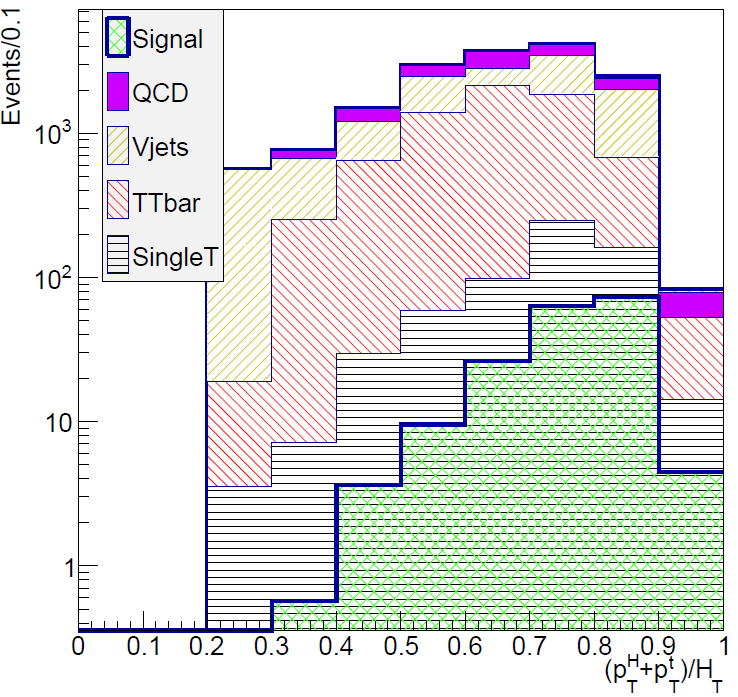
\includegraphics[width=0.45\textwidth]{figs/Pheno/RelHT.png}
    \caption{Relative total hadronic energy for backgrounds (stacked) and signal (over--imposed) normalized to 20 $fb^{-1}$ luminosity.}
    \label{fig:Var5}
  \end{center}
\end{figure}

\end{itemize}

After cut 3, but before cut 4, the \W, top and Higgs candidates are formed with the jet association method. The mass distribution of \W~and $t$ candidates is plotted in figure~\ref{fig:MWMTop}.

\begin{figure}[!Hhtbp]
  \begin{center}
    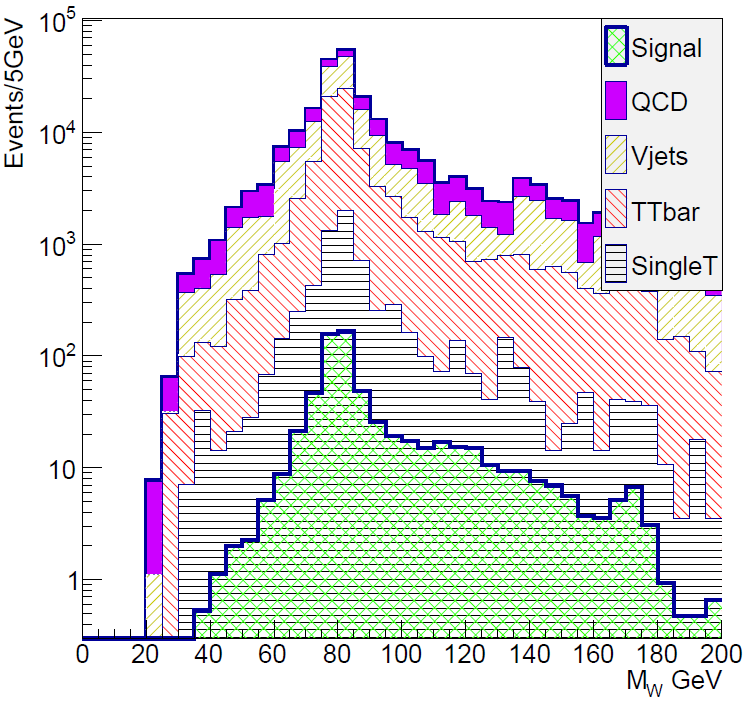
\includegraphics[width=0.45\textwidth]{figs/Pheno/MW.png}
    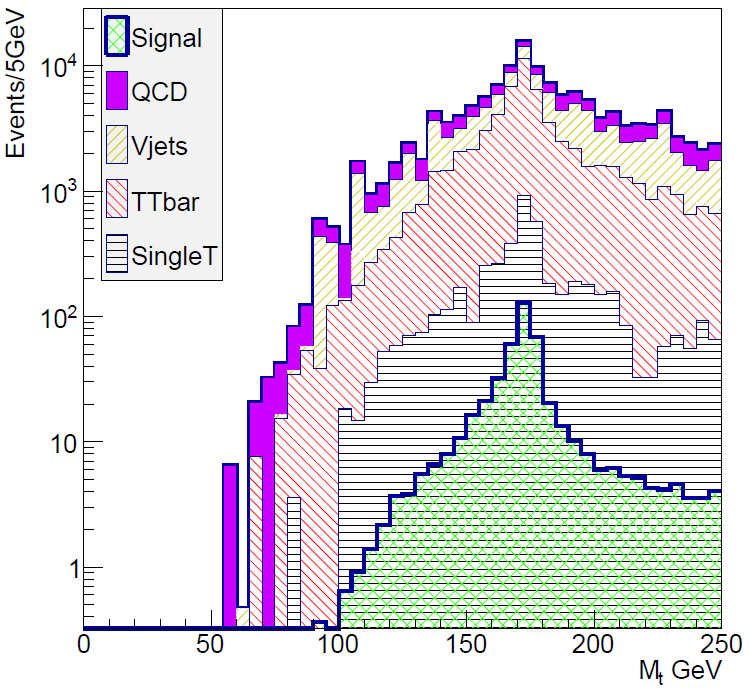
\includegraphics[width=0.45\textwidth]{figs/Pheno/Mtop.png}
    \caption{Reconstructed \W~[left] and top [right] mass for backgrounds (stacked) and signal (over--imposed) normalized to 20 $fb^{-1}$ luminosity.}
    \label{fig:MWMTop}
  \end{center}
\end{figure}

In the selection, the characteristics of the signal have been exploited in order to differentiate it from the backgrounds. Table~\ref{tab:SelEff} shows the efficiency of each cut in the procedure described above: the first line contains the number of events after the initial cut 0 normalized to an integrated luminosity of 20~fb$^{-1}$, while in the following lines the efficiencies of the cuts for signal and background samples are shown after each of the 10 cuts. The bottom line of the table contains the overall selection efficiency. 

Due to the low statistics of our samples, no numbers are quoted for the \Z+jets background (producing a \Z~boson with a high jet multiplicity is computationally very expensive). Furthermore, the inclusive \Z+jets cross section is one order of magnitude smaller than the \W+jets one and, due to the similar branching ratios and kinematics, similar efficiencies are expected as for the \W+jets background. This background is therefore ignored, and a contribution of at most with an additional 10\% of the \W+jets is assumed. In addition, from the study it was checked that the di--boson contribution is negligible. No di--boson background is quoted either.

The selection relied on angular variables that are not greatly changed by the introduction of detector effects. Correspondingly, nonetheless this study has been performed up to hadronization level in the samples production, it should not greatly change when considering detector simulation.

\begin{table}[htbH]
\begin{center}
\resizebox{\textwidth}{!}{
\begin{tabular}{l|c|c|c|c|c|c}
   & Signal & QCD & \W+jets & \ttbar & $t$+ jet & $tW$ \\ \hline
  Cut 0 & $554\pm 3$ & $203,930\pm 1,150$ & $1,015,294\pm 11,567$ &  $337,024\pm 1,608$ & $25,349\pm 300$ & $19,416\pm 469$ 
  \\ \hline
  Cut 1 & $0.91\pm 0.01$ & $0.571 \pm 0.007$ & $0.67\pm 0.02$ &  $0.439 \pm 0.005$ & $0.45 \pm 0.01$ & $0.42 \pm 0.03$ \\
  \hline
  Cut 2 & $0.92\pm 0.01$ &  $0.68\pm 0.01$ & $0.74 \pm 0.02$ &  $0.81 \pm 0.01$ & $0.61 \pm 0.02$ & $0.70 \pm 0.06$ \\
   \hline
  Cut 3 & $0.84\pm 0.01$ & $0.86 \pm 0.02$ & $0.22 \pm 0.01$ & $0.83 \pm 0.01$ & $0.82 \pm 0.04$ & $0.85 \pm 0.08$ \\
   \hline
  Cut 4 & $0.93\pm 0.01$ & $0.68 \pm 0.01$ & $0.74 \pm 0.06$ & $0.56 \pm 0.01$ & $0.49 \pm 0.03$ & $0.45 \pm 0.05$ \\
 \hline
  Cut 5 & $0.92\pm 0.01$ & $0.60 \pm 0.02$ & $0.56 \pm 0.05$ &  $0.53 \pm 0.01$ & $0.61 \pm 0.05$ & $0.56 \pm 0.09$ \\
  \hline
  Cut 6 & $0.92\pm 0.01$ & $0.61 \pm 0.02$ & $0.56 \pm 0.07$ &  $0.74 \pm 0.03$ & $0.66 \pm 0.07$ & $0.72 \pm 0.15$ \\
 \hline
  Cut 7 & $0.75\pm 0.01$ & $0.67 \pm 0.03$ & $0.67 \pm 0.11$ &  $0.71 \pm 0.03$ & $0.77 \pm 0.09$ & $0.75 \pm 0.18$ \\
  \hline
  Cut 8 & $0.87\pm 0.02$ & $0.76 \pm 0.04$ & $0.82 \pm 0.15$ &  $0.84 \pm 0.04$ & $0.77 \pm 0.11$ & $0.90 \pm 0.24$ \\
\hline
  Cut 9 & $0.91\pm 0.02$ & $0.33 \pm 0.02$ & $0.41 \pm 0.10$ &  $0.51 \pm 0.03$ & $0.52 \pm 0.09$ & $0.48 \pm 0.16$ \\
  \hline
  Cut 10 & $0.87\pm 0.02$ & $0.54 \pm 0.06$ & $0.55 \pm 0.19$ &  $0.49 \pm 0.04$ & $0.79 \pm 0.17$ & $0.72 \pm 0.31$ \\
\hline
  combined & $0.284\pm 0.005$ & $(7.5 \pm 0.5) \times 10^{-3}$ & $(3.1 \pm 0.7) \times 10^{-3}$ &  $(9.3 \pm 0.5) \times 10^{-3}$ & $(11 \pm 1) \times 10^{-3}$ & $(10.5 \pm 3) \times 10^{-3}$ \\
 \end{tabular}
}
\caption{Number of events for signal and backgrounds after the first selection cut (cut 0), and efficiencies of each stage of the cutting procedure. The errors indicated are statistical only, based on the number of events.}
\label{tab:SelEff}
\end{center}
\end{table}
%\begin{TOINCLUDE}$N-1$ plots for selection variables. Efficiency table.\end{TOINCLUDE}

\section{Results}
\label{sec:Pres}

The \Tp~peak reconstruction after full selection is shown in figure~\ref{fig:M5J}. An excess of signal events over backgrounds is found around 730~\GeVcc~for the signal over the ensemble of backgrounds. The lack of smoothness of the distribution is due to the lack of statistics in the Monte-Carlo samples for the  backgrounds, especially for \W+jets. These fluctuations due to the poor statistics can change the final estimate of the number of background events entering the peak of the signal. 

\begin{figure}[!Hhtbp]
  \begin{center}
    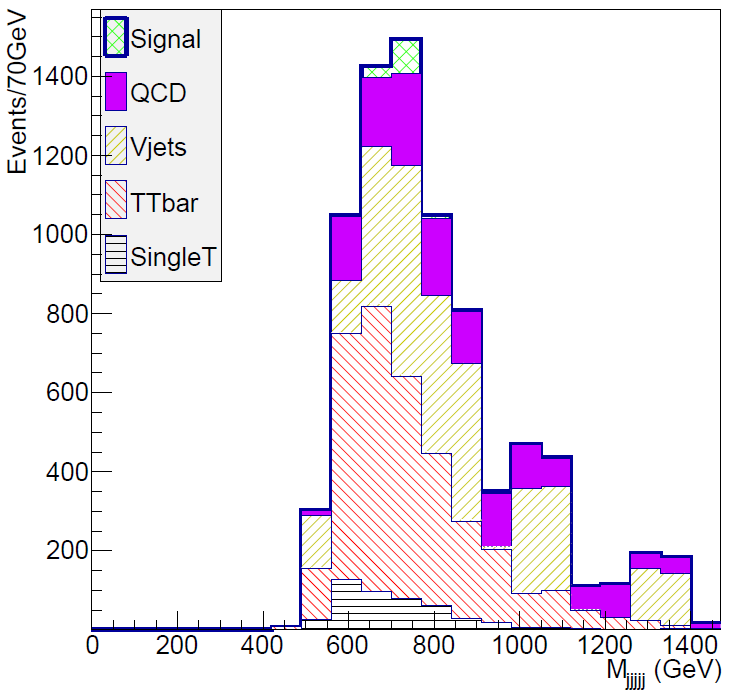
\includegraphics[width=0.45\textwidth]{figs/Pheno/Final.png}
    \caption{Reconstructed \Tp~mass after all cuts for backgrounds and signal (stacked) normalized to 20~$fb^{-1}$ luminosity. Signal peak is visible on top of the sum of backgrounds.}
    \label{fig:M5J}
  \end{center}
\end{figure}

From the peak reconstruction, the number of events falling into a window of $20$~GeV around the \Tp~mass was selected, i.e. within $710 < M_{jjjjj} < 750$~GeV. The number of events contained in this window, for each process, is listed in table~\ref{tab:events}. An enhanced signal over background ratio is obtained, with:
\begin{equation}
\frac{S}{\sqrt{S+B}}=2.0\pm 0.3\,, \qquad \mbox{and} \quad \frac{S}{B}=0.06\pm 0.02\,. 
\end{equation}

To the quoted uncertainties, uncertainties linked to the cross section calculation for the signal should be added, PDF's and possible loop contributions. From similar studies and analyses done by ATLAS and CMS collaborations the uncertainties linked to these sources are not bigger than 10\% to 15\% (see for instance \cite{Aad:2011yn}), therefore their inclusion should not change significantly the conclusions of this study.

\begin{table}[tb]
\begin{center}
\begin{tabular}{l|c|c|c|c}
 & \multicolumn{2}{c|}{unweighted events}  & \multirow{2}{*}{weight} & weighted  \\
 & after Cut 10 & in mass window & & events \\
 \hline
 Signal & $8601$ & $3780$ & $0.018$ &$69 \pm 1$ \\
 \hline
   $t \bar{t}$ & $409$ & $57$ & $7.7$ & $437 \pm 58$ \\
 $W$+jets & $24$ & $3$ & $132$ & $395 \pm 228$ \\
 $QCD$ & $235$ & $34$ & $6.48$ & $220 \pm 38$ \\
 $tW$ & $18$ & $3$ & $11.3$ & $34 \pm 20$ \\
 $t$+ jet & $75$ & $7$ & $3.55$ & $25 \pm 9$ \\
  \hline
  total background & & & & $1112 \pm 352$ \\
\end{tabular}
\caption{Number of signal and background events from utilized MC samples: in the first column the simulated events that pass all kinematic cuts, in the second column the events that fall in the mass window ${710<M_{jjjjj}<750}$~\GeVcc, finally in the fourth column the number of weighted events in the mass window normalized to the physical cross section (the applied weight is listed in the third column). All the errors are statistical only. For the total background, the linear sum of errors was considered.} \label{tab:events} 
\end{center}
\end{table}

As final remark, the signal sample used for the study was generated with a \Tp~width of 1~\GeVcc. However, the theoretical model predicts a width of 11~\GeVcc~for the benchmark point that has been used. For this larger width, an opening up to 30~\GeVcc on the integration window is needed to include 2-$\sigma$ of the signal. Nonetheless, with these changes the estimator $S/\sqrt{S+B}$ does not change significantly within the statistical error. Then, the conclusion of the study does not change taking into account the larger \Tp~width.

In conclusion, this study shows a plausible selection in order to perform a data analysis to test a hypothetical \Tp~that decays into a top quark and a Higgs boson in the full hadronic channel. Moreover this study shows, how mixed couplings of VLQ to light and heavy quark generations enhance the VLQ production cross section; and also give specific signatures to search for these VLQ beyond SM particles. 

It is important to stress that the present study, as the CMS analysis that will be presented afterward, rely in a VLQ model that has been poorly explored in experiments. This model allows the VLQ to be mixed to the three generations of SM quarks, enhancing the production cross section in proton-proton collisions. The most common VLQ models assume that the top-partner mixes preferentially to third SM-quark generation. The model used in this work represents then a generalization with respect to the most widely used models in the literature.

In chapter~\ref{chap:search}, a data analysis using data collected by CMS experiment during run 1 is presented. The present work concludes with the experimental limits set on this model.

%\begin{TOINCLUDE}Expected yields table. Final M5J plot.\end{TOINCLUDE}
